\documentclass{article}
\usepackage{graphicx}
\usepackage[brazilian]{babel}
\usepackage[utf8]{inputenc}
\usepackage[T1]{fontenc}

\graphicspath{ {images/} }
 
\title{Arquitetura do Atari 2600}
\author{Rodrigo Junger}
\date{ }

\renewcommand*\contentsname{Sumario}

 
\begin{document}
 
\maketitle
 
\tableofcontents


\renewcommand{\abstractname}{Introdução}
\begin{abstract}
Inicialmente chamado de Atari VCS, o Atari 2600 é um console 8bit lançado em setembro de 1997. Ele possui um processador 8-bit, um chip gráfico chamado de TIA (Television Interface Adapter) e um chip chamada PIA (Peripheral Interface Adaptor) com timers programáveis e 128 bytes de memória RAM mapeados nos endereços 80 até FF da memória. A memória do PIA é geralmente usada para guardar variáveis.
\end{abstract}

\section{Processador}
\paragraph{}
O processador do Atari 2600 é o 6507, que é basicamente uma versão menor e com menos pinos do 6502. Ele opera com uma frequência de 1.19Mhz e tem apenas 6 registradores, cinco de 8 bits e um especial de 16 bits usado para o PC.

\subsection{Registradores}

\begin{center}
	\begin{tabular}{| l | l | l |}
	\hline
	Bits & Nome & Uso \\ \hline
	8 & A & Acumulador \\ \hline
	8 & X & Registrador de uso geral X \\ \hline
	8 & Y & Registrador de uso geral Y \\ \hline
	8 & S & Stack pointer \\ \hline
	8 & P & Flags (Processor Status Register) \\ \hline
	16 & PC & Program Counter \\ \hline
	\end{tabular}
\end{center}

\subsubsection{A}
Operações aritméticas como soma e adição e algumas operações binárias como OR, AND e XOR só podem ser feitas com esse registrador, um detalhe interessante é que o 6502, assim como a maioria dos processadores dessa época, não tem operações de divisão e multiplicação, o programador tem que "emular" as duas com somas, subtrações e comparações.

\subsubsection{X e Y}
São registradores mais gerais, a única operação aritmética que pode ser feita diretamente nesses registradores é a adição e a subtração por 1, por isso são muito usados como contadores em loops.

\subsubsection{S}
Stack Pointer. Ao contrario do que normalmente acontece em computadores modernos, a stack do Atari começa de cima (normalmente do endereço FF) e cresce para baixo.

\subsubsection{P}
Todas as flags como overflow e zero são guardadas nesse registrador, a tabela abaixo mostra qual flag cada bit desse registrador guarda e o que ela significa.

\begin{center}
	\begin{tabular}{| l | l | l | l |}
	\hline
	Bit & Nome & Uso & Explicação \\ \hline
	0 & C & Carry & (0=Sem carry, 1=Carry) \\ \hline
	1 & Z & Zero & (0=Não zero, 1=zero) \\ \hline
	2 & I & IRQ Disable & (0=IRQ Habilitado, 1=IRQ Habilitado) \\ \hline
	3 & D & Modo decimal & (0=Normal, 1=Modo BCD para os opcodes ADC e SBC) \\ \hline
	4 & B & Break flag & (0=IRQ/NMI, 1=RESET ou opcode BRK/PHP)\\ \hline
	5 & - & Não utilizado & - \\ \hline
	6 & V & Overflow & (0=Sem Overflow, 1=Overflow)\\ \hline
	7 & N & Negative & (0=Positivo, 1=Negativo)\\ \hline
	\end{tabular}
\end{center}



\subsubsection{PC}
Guarda o endereço de memória da próxima instrução que será executada, é alterado por instruções que fazem branch como JMP, JSR e BCS.


\subsection{Assembly 6502}
\paragraph{}
O 6502 Possui apenas 56 instruções sempre nomeadas com 3 letras e que podem receber no máximo 1 argumento, essas instruções podem ter de 1 a 3 bytes dependendo do tipo da instrução e do modo de endereçamento usado.


\subsection{Modos de endereçamento}
\paragraph{}
Um dos fatores que contribui para a grande flexibilidade do 6502 são os diversos modos de endereçamento existentes, um modo de endereçamento muito importante é o chamada de "Zero Page", este modo é usado para endereçar apenas os primeiros 256 bytes da memória e é importante pois economizamos memória e ciclos do processador, já que a instrução resultante usa apenas dois bytes.


\section{TIA (ntsc)}

\paragraph{}
O que realmente da vida aos jogos do Atari 2600 é um chip chamado de Television Interface Adaptor, esse chip cuida da imagem e do áudio que são enviados para a TV, alem de ser responsável por ler o input dos controles.
\paragraph{}
Cada frame tem 262 linhas horizontais de 228 pixels, e o Atari processa 60 frames por segundo, isso significa que o clock é de aproximadamente 3.58 MHz, ou o triplo do clock do processador principal. Temos então que cada linha dura 76 ciclos de maquina do processador principal.

\subsection{Linha}
Toda linha começa com 68 pixels de Blaning Horizontal seguidos por 160 pixels normais.

\subsection{Frame}
O frame é formado por 262 linhas nessa ordem: 
\begin{itemize}
	\item 3 Linhas de VSYNC
	\item 37 Linhas de VBLANK
	\item 192 Linhas da imagem que vai aparecer na TV
	\item 30 linhas de overscan
\end{itemize}

Como mostra a figura 1, boa parte da imagem é "comida". O motivo disso é compatibilidade, nessa época não existia um padrão exato para mandar imagens para a TV e os engenheiros da atari concluíram que essa era a maneira que funcionaria melhor com todas as TVs.

\begin{figure}[h]
	\caption{Frame do atari}
	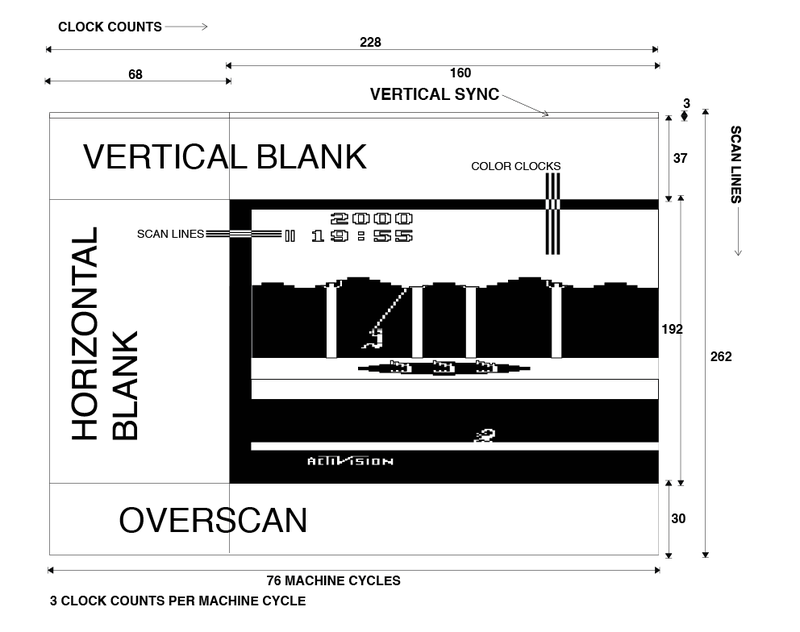
\includegraphics[width=\textwidth]{televisionscreen}
\end{figure}

\subsection{Desenhando na tela}
\paragraph{}
A parte mais complexa e também a mais importante é desenhar na tela, como na época memoria RAM era extremamente cara, o Atari não tinha um framebuffer, tudo era feito linha por linha e as únicas coisas (sem contar as inúmeras gambiarras) que podíamos desenhar eram 2 jogadores, 2 misseis, uma bola, um campo (playfield) e o background que é apenas a cor desenhada quando não existe nada de especial num determinado pixel. Os únicos objetos que podem se mover são os jogadores, os misseis e a bola; o playfield e o background são estáticos.
\subsubsection{Posicionamento vertical de objetos}
\paragraph{}
Para posicionar um objeto verticalmente, basta apenas habilitar o objeto na(s) linha(s) que você deseja que o objeto apareça, isso é feito de formas diferentes para objetos diferentes, no caso dos jogadores basta setas os 8bits de informação para 0, já os misseis e a bola tem um registrador de enable que pode ser 1 ou 0.
\subsubsection{Posicionamento horizontal de objetos}
\paragraph{}
A posição horizontal de um objeto é um pouco mais complicada, é preciso escrever no registrador de RESET do objeto (RESP, RESM, RESBL) quando ele está no pixel desejado, isso vai setar a posição do objeto para essa posição, para movimentos pequenos é possível usar os registradores de movimentação (HMP, HMM, HMBL), o objeto pode se movimentar de -7 a +8 pixels cada vez que algo é escrito no registrador HMOVE, isso pode ser feito mais de uma vez por linha para mover mais que o limite ou para criar efeitos interessantes com repetição.



%\section{PIA}
%Coisas sobre o PIA
 
\end{document}